%
\chapter{提案手法}
%
\section{モデル概観}
この章では,提案モデルがもつ複合特徴量抽出器とニュース分類器について紹介する.
その後にこの2要素を統合して転移学習が可能な表現を学習する方法について説明する.
% 最後に,詳細なアルゴリズムフローを付加する. 
今回提案したモデルは,以下の図\ref{fig:model}の通りである.

提案モデルの目的は,画像と文章で発信された情報に対して,
正しいニュースか・フェイクニュースか・ジョークニュースかを分類するために,
必要な特徴表現を学習することであった.
提案モデルは複合特徴量抽出器とニュース分類器の大きく2部分に分けることができた.
まず複合特徴量抽出器は,今回扱う情報が文章と画像を含むため,
各メディアに対して特徴化する抽出器があった.
その後それぞれの特徴を1つに連結し,複合特徴を形成した.
複合特徴はニュース分類器に送られ,最終的には3カテゴリのどれに該当するかが判断された.
% 
\begin{figure}[H]
    \centering
    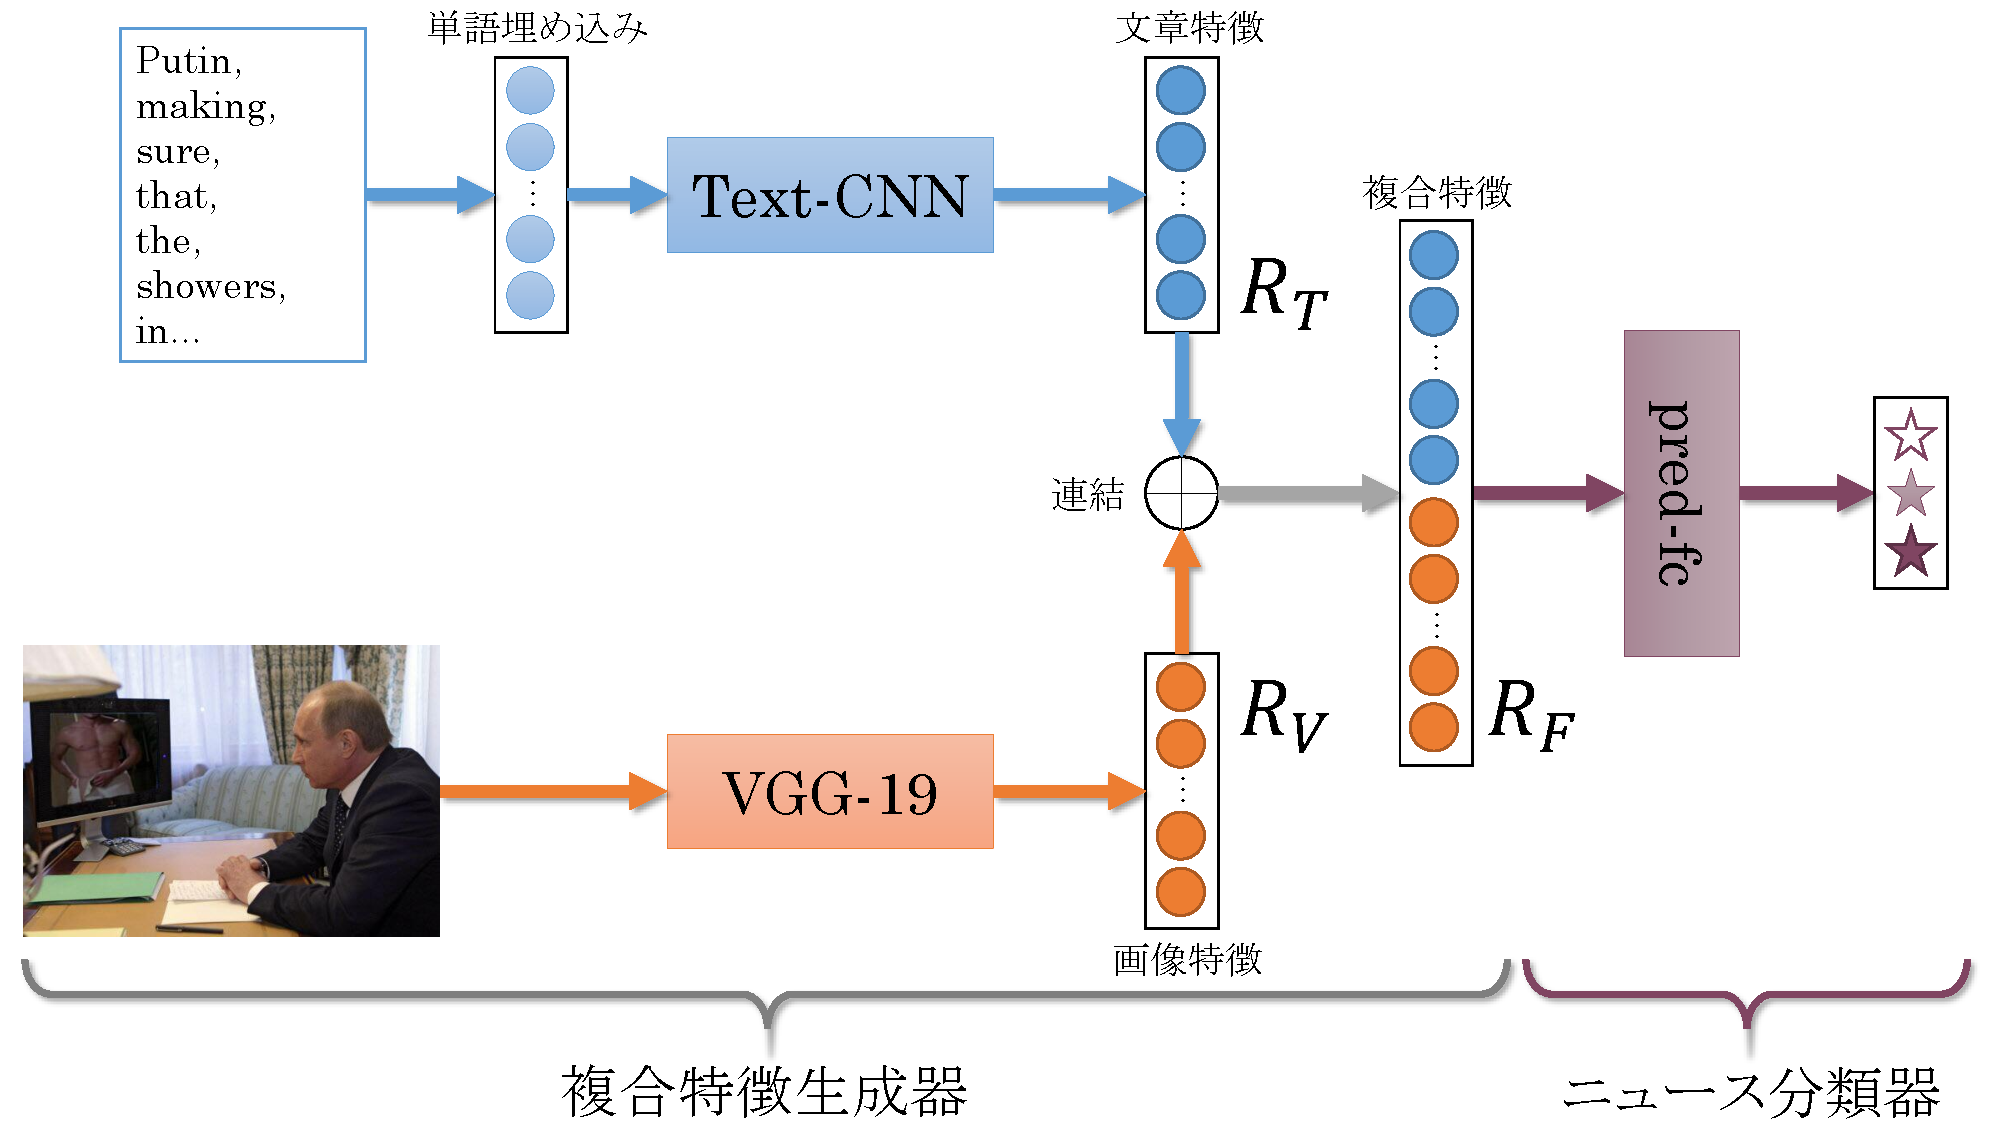
\includegraphics[width=0.8\linewidth]{images/methodology.pdf}
    \caption{提案モデル図.青: 文章特徴量抽出器,橙: 画像特徴抽出器,紫: ニュース分類器.}
    \label{fig:model}
\end{figure}
%
\section{複合特徴抽出器}
%
\subsection{文章特徴} \label{subsec:text}
文章特徴は,入力に英語の投稿をスペース毎に分割した英単語の連続リストをもった.
まずは単語を単語埋め込みでベクトル化した.
その後単語の羅列から分類に有効な情報を得るために,文章特徴を抽出する核としてCNN
(convolutional neural networks: 畳み込みニューラルネットワーク)を採用した.
CNNはコンピュータビジョンやテキスト分類などの多くの分野で効果的であることが示されていた
\cite{collobert2011natural,KalchbrennerACL2014}.
図\ref{fig:model}の通り,提案手法ではCNNの発展形であるテキストCNN(Text-CNN)\cite{DBLP:journals/corr/Kim14f}を採用した.
テキストCNNの構造は図\ref{fig:text-cnn}の通りである.
複数のウィンドウで畳み込むことで,様々な角度から特徴を抽出することを実現した.
\begin{figure}[H]
    \centering
    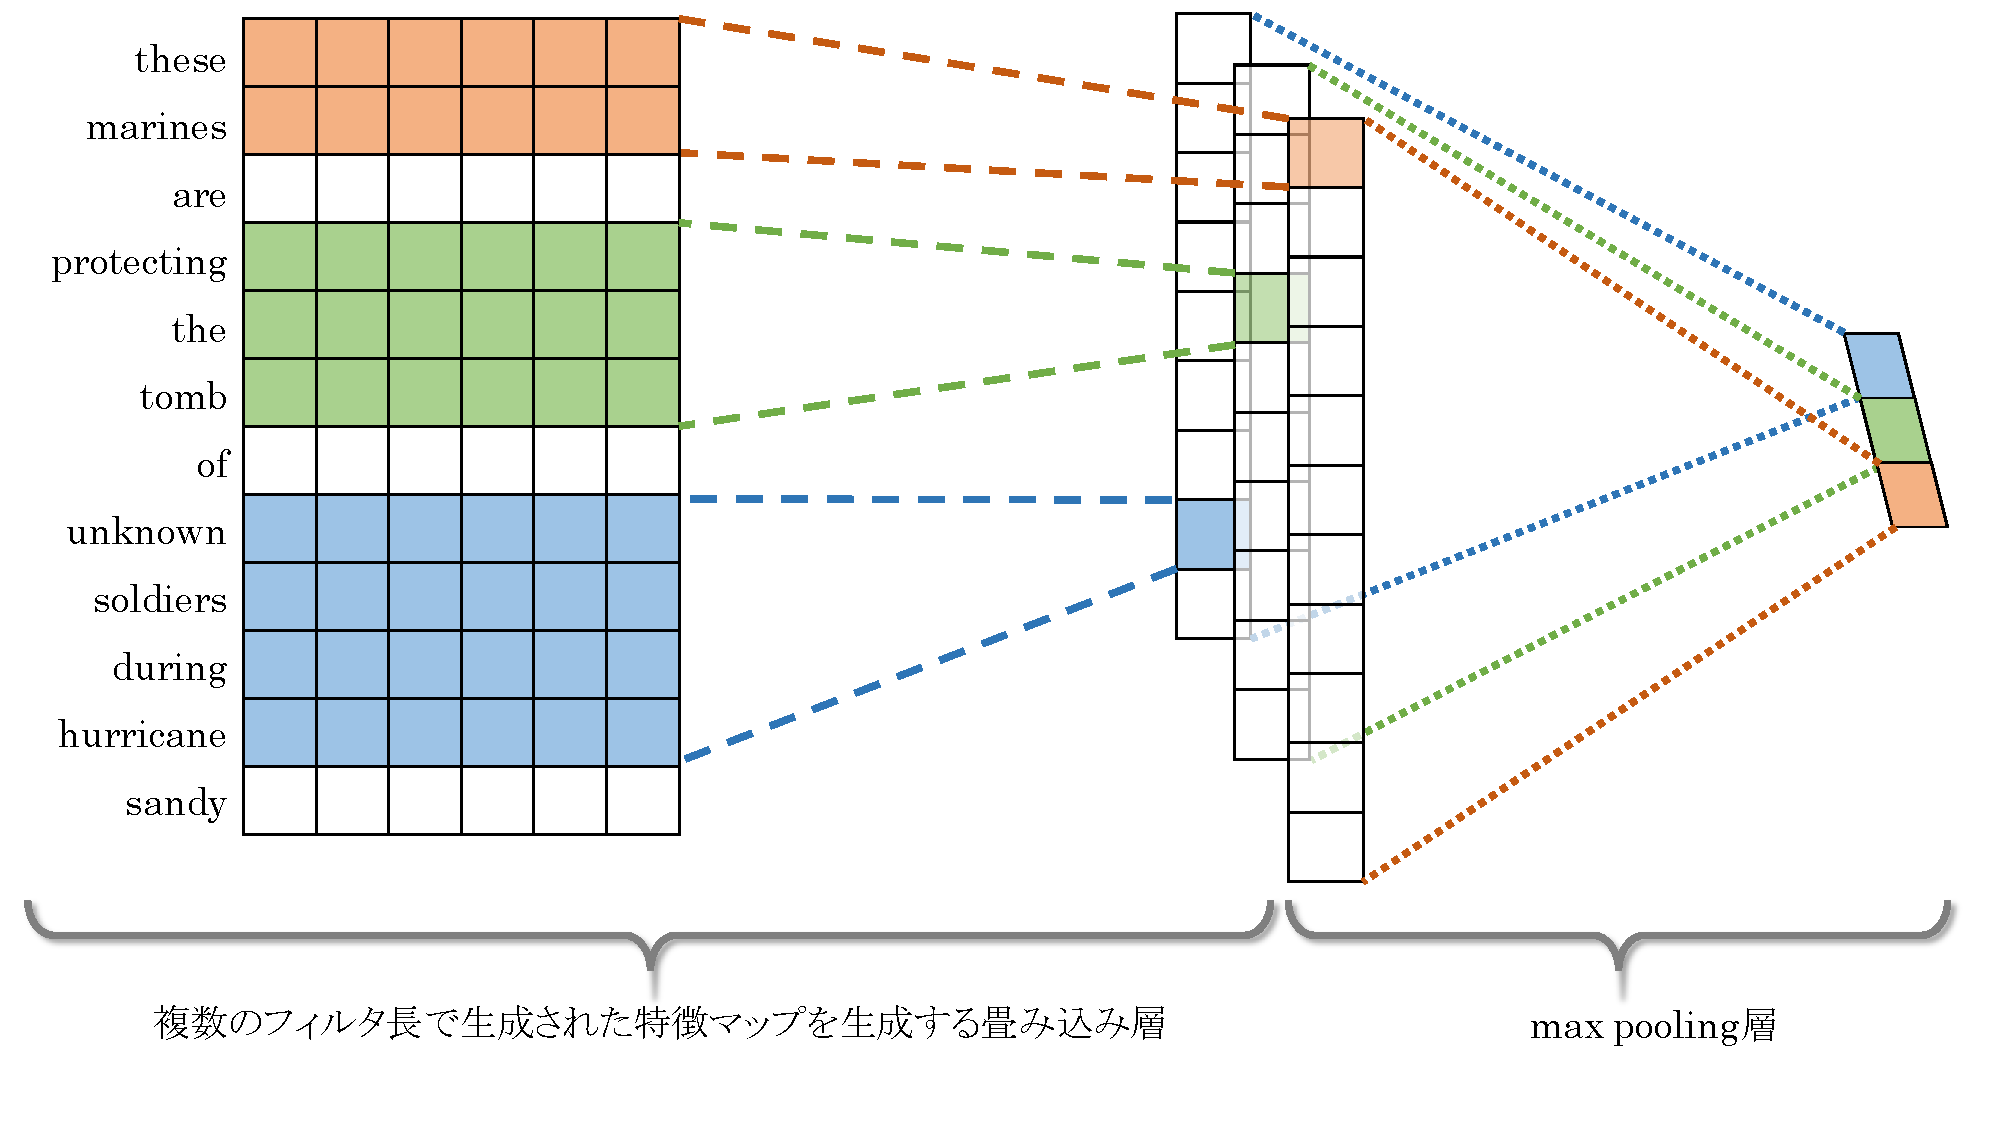
\includegraphics[width=\linewidth]{images/text-cnn.pdf}
    \caption{テキストCNNの図.Wangらの研究\cite{Wang:2018:EEA:3219819.3219903}を参考に作成.}
    \label{fig:text-cnn}
\end{figure}

具体的な手法では,EANNが採用したテキストCNN同じ流れを汲み\cite{Wang:2018:EEA:3219819.3219903},
最終の全結合層の隠れ層に独自にdropoutを採用した形をとった.
dropoutはHintonらによって提案された手法\cite{JMLR:v15:srivastava14a}で,
学習時に指定された確率で無作為に$W_{tf}$内の要素を無効化(0に)してモデルの自由度を制限することで,
モデルが訓練データセットに特化しすぎて汎用性が失われる過学習に繋がりにくくなる利点が報告されたものであった.
%
\subsection{画像特徴}
画像から効率的に特徴を抽出するために,当研究では事前学習済みのVGG19\cite{DBLP:journals/corr/SimonyanZ14a}を起用した.
VGG19は畳み込み16層と全結合層3層から形成され,最終的には1000次元の特徴ベクトルが出力される.
当研究では最終の全結合層のみ改変し,文章特徴のベクトル次元数と同じ数の次元をもつベクトルを出力されるようにした.
また改変した最終全結合層以外は,過学習を防ぐために事前学習の状態を維持することにした.

こうして文章特徴・画像特徴が抽出され,最終的には2つの特徴ベクトルを1つに連結したものが複合特徴である.
連結された複合特徴は,次元数が文章・画像特徴の次元数を足した数となる.
%
\section{ニュース分類器}
%
複合特徴はニュース分類器(図\ref{fig:model}内`pred-fc'が該当)にて正しいニュース・フェイクニュース・ジョークニュースとして分類された.
具体的には隠れ層を含む全結合層とsoftmaxから形成され,最終的な分類が行われた.
モデルの目的は自動で正確に正しいニュース・フェイクニュース・ジョークニュースを分類することである.
そのため正解ラベルを使用して,クロスエントロピー誤差を損失として算出する.
このあと,当研究がベースとしたWangらの研究では確率的勾配降下法(SGD: Stochastic Gradient Descent)
によってパラメータを更新していたが,
当研究では2015年にDiederik P. Kingmaらが提唱したAdamという手法\cite{DBLP:journals/corr/KingmaB14}
を用いてパラメータを更新することにした.
%

